
%% simple table 
% https://www.youtube.com/watch?v=gpzeV-N7wfk&list=PLNnwglGGYoTtW7o4PHFOSWGevcdFa3v3D&index=6 

%\begin{table}
%  \caption{A stunning table}
%  \label{tbl:excel-table}
%  \includegraphics[width=\linewidth]{excel-table}
%\end{table}

\cleardoublepage

\addcontentsline{toc}{chapter}{\numberline{}Étude expérimentale}
\addtocontents{lof}{\textbf{Étude expérimentale}}

\setcounter{chapter}{5}
\setcounter{section}{0}
\setcounter{figure}{0}

\begin{center}
	\Huge\textbf{Étude expérimentale}
\end{center}

\section{Introduction}
Dans le chapitre précédent, nous avons présenté en détail les approches que nous avons proposées pour la résolution du problème de l’arbre dominant (DTP). Nous allons présenter dans ce qui suit une étude expérimentale effectuée pour comparer les résultats des approches proposées avec d’autres approches développées pour la résolution du DTP. Nous clôturons avec une conclusion.


\section{Environnement de travail}

\subsection{Environnement matériel}
Pour les tests effectués nous avons utilisé une machine. Les caractéristiques de  machine sont données dans la figure \ref{fig:CMU}.

\begin{figure}[H]
	\centering
	
\includegraphics[width=16cm,height=7cm]{Chap5/1.png}
	\caption{Caractéristiques de la machine utilisée}
	\label{fig:CMU}
\end{figure}

\subsection{Environnement logiciel}
Nous avons opté pour le langage Java pour la programmation, car il offre une grande flexibilité et facilite l’implémentation qui est due au fait qu’il soit totalement orienté-objet.

\textbf{IDE :}
L’environnement de développement choisit est IntelliJ IDEA, spécialement dédié au développement en utilisant le langage Java. Il est proposé par l’entreprise JetBrains et est caractérisé par sa forte simplicité d’utilisation et les nombreux plugins et extensions qui lui sont dédiées.

\section{Jeux de données utilisées}
Afin de tester l'approche proposée, nous avons opté pour l'utilisation de fichiers benchmark qui vont représenter des instances du problème. Les différentes instances sur lesquelles notre étude s'est portée sont dérivées à partir des mêmes benchmarks de \cite{sundar2013new}. Une instance est considérée comme un graphe de disques, G = ( V, E ) où chaque disque représente la plage de transmission de chaque nœud. Le poids de chaque arête $e_{uv} \in E $ est défini sous la forme w ( u, v ) = $d_{uv}^2$, où $d_{uv}$  est la distance euclidienne entre deux nœuds u et v. L'hypothèse est que tous les nœuds sont répartis de manière aléatoire dans une zone de $500m * 500m $  et la plage de transmission de chaque nœud est de 100 m.


\section{Expérimentation}
Pour montrer l'efficacité de l'approches proposées nous ne nous sommes pas limité à des instances de problème ayant un certain nombre de nœuds.

Nous nous avons effectué cela pour une large plage de nombre de nœuds (50 - 500).

Pour ACO, nous avons utilisé une population de 15 fourmis. Nous avons utilisé $\alpha = 1 \, , \, \beta = 1 \, , \, p = 0.05 \, , \, P_0 = 0.1 $. Toutes les valeurs de phéromone initiales sont égales à 0,05. Pour BBO et GA, la taille de la population est de 20 individus. Quant à l’approche de coopération,  nous avons utilisé 0.5 comme probabilité initiale et 0,1 pour la valeur de  \( \alpha \).

Pour toutes les instances du test, nous avons opté pour 100 itérations pour chacune des approches proposées. Nous avons jugé que ce nombre d'itérations est suffisant pour une qualité quasi optimale de la solution. Donner plus d'itérations à nos approches que celles mentionnées ci- dessus n'aura que peu d'impact sur la qualité de la solution. 

Toutes ces valeurs de paramètres sont choisies empiriquement. Ces valeurs de paramètres donnent de bons résultats pour la majorité des instances de test.

\subsection{Étude comparative}
Afin de mener à bien une étude comparative entre nos approches et d’autres travaux effectués pour la résolution du DTP, nous avons gardé approximativement le même nombre d’évaluations de la fonction objectif.

Dans le but d’assurer l’intégrité des résultats, nous avons effectué un total de 20 exécutions pour chacune des instances. Les résultats d’exécutions de nos approches (ACO, BBO, GA et la méthode coopérative) sur les instances citées auparavant, sont illustrés dans le Tableau \ref{tab:1}.

Dans le Tableau  \ref{tab:1}, les lignes correspondent aux différentes instances étudiées, quant aux colonnes, elles représentent, pour chaque approche : la meilleure solution obtenue (colonne BS), la moyenne de toutes les solutions obtenues sur les 20 exécutions (colonne AVG), le nombre d’évaluations nécessaire pour trouver la meilleure solution (colonne NBV) et la colonne qui représente le temps d’exécution de chaque métaheuristique en seconde (colonne sec). 
Notez que les meilleures valeurs sont indiquées en gras dans les tableaux comparatifs.


\begin{table}[H]
	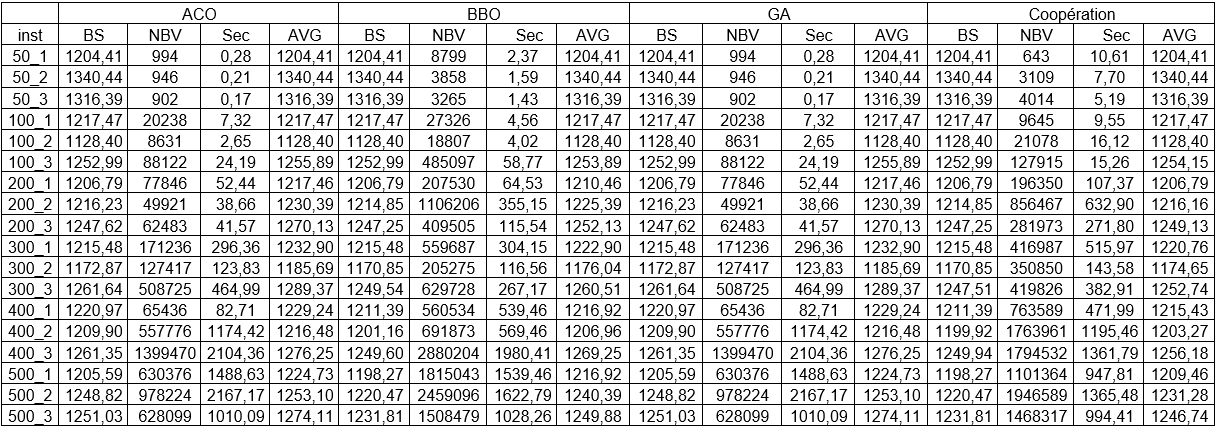
\includegraphics[width=17cm,height=7cm]{Chap5/t1.png}
	\caption{Résultats d’exécutions des  approches proposées}
	\label{tab:1}
\end{table}


\subsubsection{Comparaison de la méthode coopérative avec les autres approches}
Dans ce qui suit nous allons présenter une comparaison entre notre approche coopérative et les autres approches que nous avons développées. Cette comparaison a pour but de montrer l’efficacité de notre approche coopérative par rapport aux approches développées. 

\begin{enumerate}[label=\alph*)]
	\item \textbf{Avec l’approche ACO}\\
	D’après le graphe de la figure \ref{fig:DEMACOMC} et les résultats présentés dans le tableau \ref{tab:2}, les résultats des deux approches sont similaires pour les 11 premières instances. La meilleure solution (BS) obtenue par l’ approche coopérative  est meilleure que celle obtenue par ACO pour les sept  (7) dernières instances. Il faut également noter que la qualité moyenne des solutions (AVG) obtenue par la méthode de coopération est  meilleure que celle d’ACO pour la majorité des instances du problème. Comparé à ACO, le nombre d’évaluation donnée par  l’approche de coopération est relativement faible. Enfin,  le temps d’exécutions  d'ACO en général est moins important.

\begin{table}[H]
	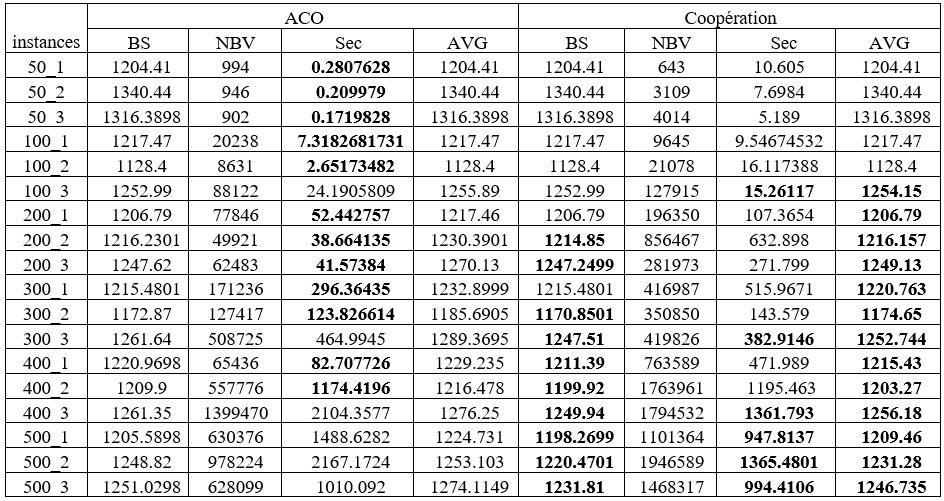
\includegraphics[width=15cm,height=8cm]{Chap5/t2.png}
	\caption{Résultats d’exécutions d’ACO et la méthode de coopération}
	\label{tab:2}
\end{table}

\begin{figure}[H]
	\centering
	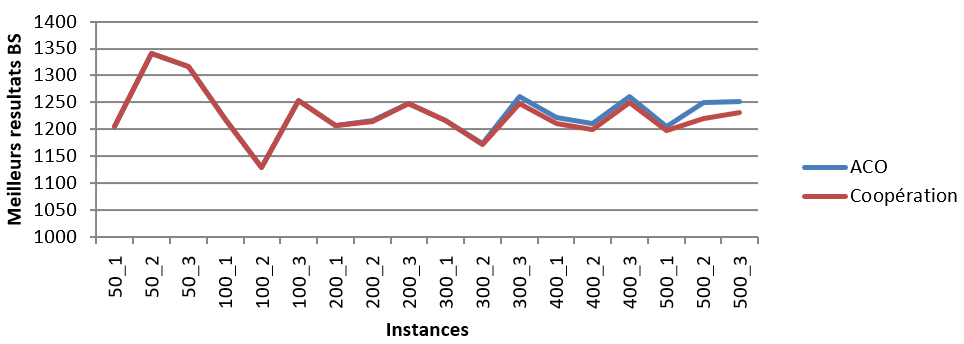
\includegraphics[width=16cm,height=7cm]{Chap5/2.png}
	\caption{Diagrammes d’exécutions de la méthode ACO et la méthode coopérative}
	\label{fig:DEMACOMC}
\end{figure}

	\item \textbf{Avec l’approche BBO}\\
D’après le graphe de la figure \ref{fig:DEMBBOMC} les deux approches sont similaires. De même, en analysant le tableau \ref{tab:3}, la meilleure solution (BS) obtenue par la méthode BBO et celle obtenue par l’approche de coopération est pratiquement la même.

Concernant les moyennes des solutions (AVG), celles obtenues par l’approche coopérative sont de meilleures qualités par rapport à celles obtenues par BBO.

Pour ce qui est du nombre d'évaluations celui de l’approche coopérative est négligeable comparé à l’autre approche.

\begin{table}[H]
	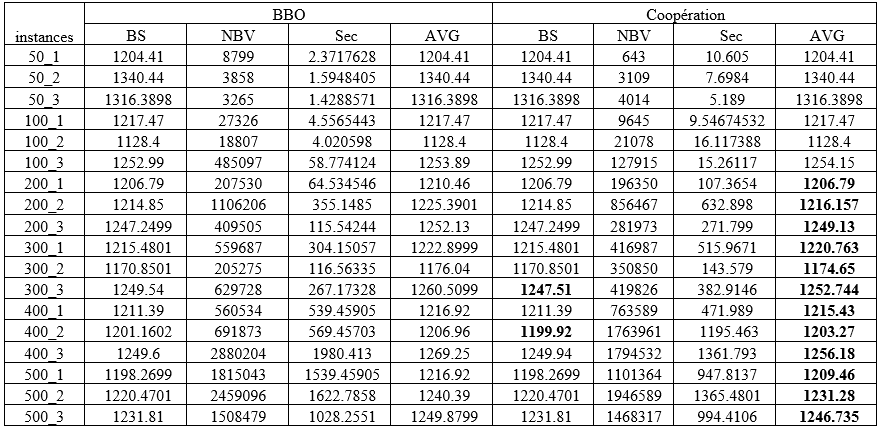
\includegraphics[width=15cm,height=8cm]{Chap5/t3.png}
	\caption{Résultats d’exécutions de BBO et la méthode de coopération}
	\label{tab:3}
\end{table}

\begin{figure}[H]
	\centering
	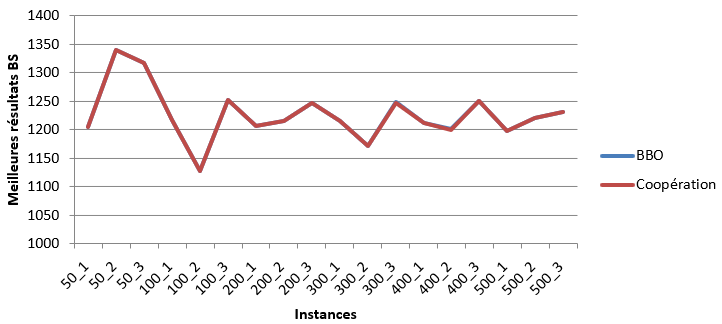
\includegraphics[width=16cm,height=7cm]{Chap5/3.png}
	\caption{Diagrammes d’exécutions de la méthode BBO et la méthode coopérative}
	\label{fig:DEMBBOMC}
\end{figure}

	\item \textbf{Avec l’approche GA}\\	
D’après le graphe de la figure \ref{fig:DEMGAMC} et les résultats présentés dans le tableau \ref{tab:4}, les deux approches sont similaires pour les 11 premiers instances, la meilleure solution (BS) obtenue par l’ approche coopérative  est meilleure que celle obtenue par GA pour les sept  (7) dernieres instances. Il faut également noter que la qualité moyenne des solutions (AVG) obtenue par la méthode de coopération est de meilleure qualité que celle obtenue par GA pour toutes les instances du problème. Comparé à GA, le nombre d’évaluation donnée par  l’approche de coopération est relativement faible.

\begin{table}[H]
	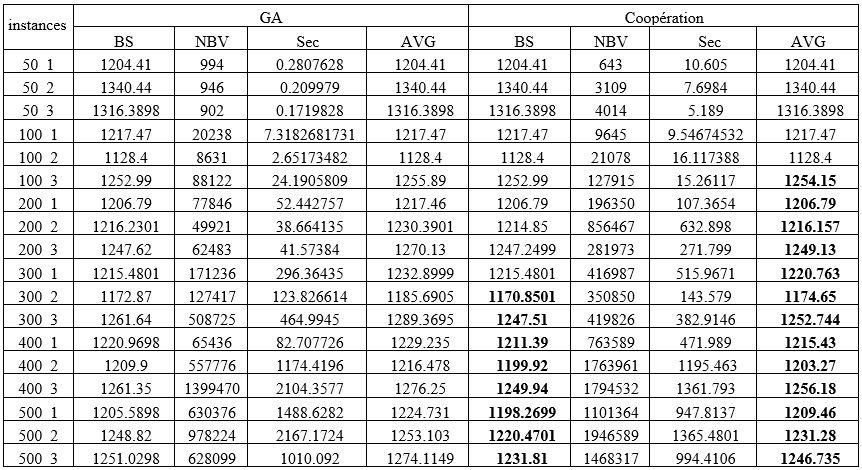
\includegraphics[width=15cm,height=8cm]{Chap5/t4.png}
	\caption{Résultats d’exécutions de GA et la méthode de coopération}
	\label{tab:4}
\end{table}

\begin{figure}[H]
	\centering
	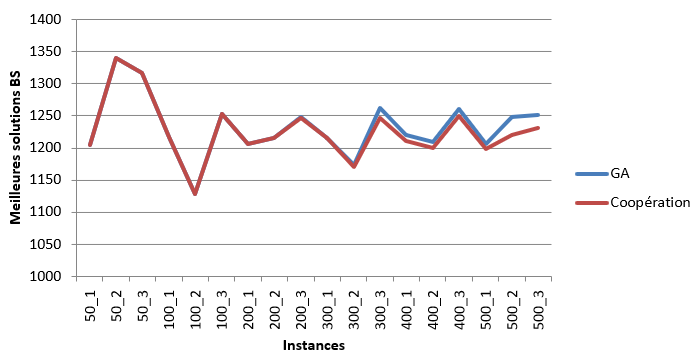
\includegraphics[width=16cm,height=7cm]{Chap5/4.png}
	\caption{Diagrammes d’exécutions de la méthode GA et la méthode coopérative}
	\label{fig:DEMGAMC}
\end{figure}


\end{enumerate}


\subsubsection{Comparaison de la méthode coopérative avec les travaux liés au DTP}
Afin de monter l’efficacité et la robustesse de notre approche coopérative, Nous l’avons comparé à deux techniques méta-heuristiques basées sur un essaim dans la littérature, à savoir ACO\_DT [55] et ABC\_DT [54], et une autre méta-heuristique SSGA \cite{sundar2014steady} .


\begin{enumerate}[label=\alph*)]
	\item \textbf{Comparaison de  la méthode coopérative avec ABC\_DTP}\\
	Dans le tableau V.5 notre méthode de coopération est meilleure sur 5 instances et similaire pour 11 instances sur 18 instances. En termes de solution moyenne, on remarque que la coopération est meilleure sur 8 instances, de moindre qualité pour 8 autres instances et est similaire pour 2 instances.
	
\begin{table}[H]
	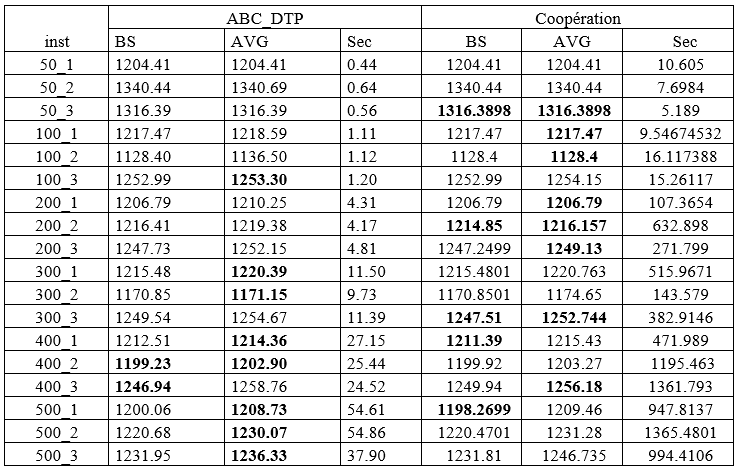
\includegraphics[width=15cm,height=8cm]{Chap5/t5.png}
	\caption{Résultats d’exécutions de ABC\_DTP et la méthode de coopération}
	\label{tab:5}
\end{table}

	\item \textbf{Comparaison de  la méthode coopérative avec ACO\_DT}\\
	D’après le tableau \ref{tab:6}, il est bien clair que la méthode de coopération est la meilleure technique en terme de la meilleure solution ainsi que la qualité moyenne de la solution. La méthode de coopération a pu générer un BS de meilleure qualité que celui d’ACO\_DT pour la plupart des instances (huit instances) et une solution de moindre qualité par rapport à celle d’ACO\_DT. Pour le reste des instances les résultats sont similaires pour les deux techniques. Concernant les moyennes des solutions obtenues (AVG), la coopération donne de meilleurs résultats que ACO\_DT dans 13 instances, et fournit une solution de moindre qualité dans une seule instance. Les résultats sont similaires pour le reste des instances (6 instances).
	
\begin{table}[H]
	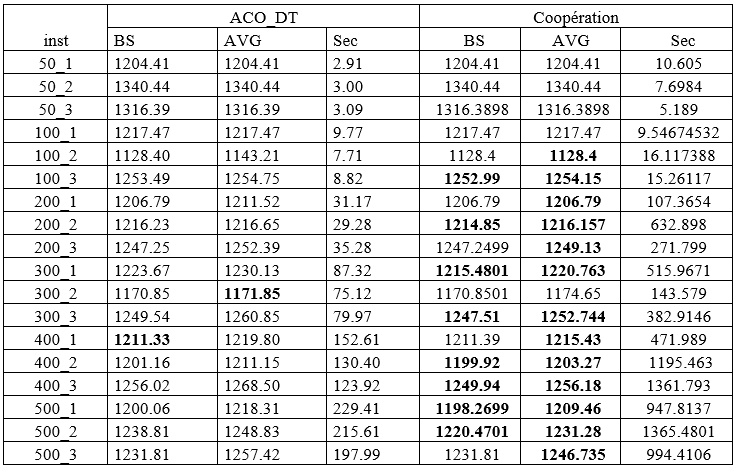
\includegraphics[width=15cm,height=8cm]{Chap5/t6.png}
	\caption{Résultats d'exécutions d'ACO\_DT et la méthode de coopération}
	\label{tab:6}
\end{table}


	\item \textbf{Comparaison de  la méthode coopérative avec SSGA}\\
	Comme le tableau \ref{tab:7} le montre, parmi les quatre  instances, la meilleure solution (BS) obtenue par la coopération est similaire à celle obtenue par SSGA dans 11 instances et est moins bonne que le BS trouvé par SSGA dans une seule instance (400\_3).
	
Concernant les moyennes des solutions (AVG), celles obtenues par la coopération sont similaires à celles obtenues par SSGA dans deux instances (50\_2 et 300\_2) et sont de moindre qualité par rapport à SSGA dans une seule instance (100\_3).

	
\begin{table}[H]
	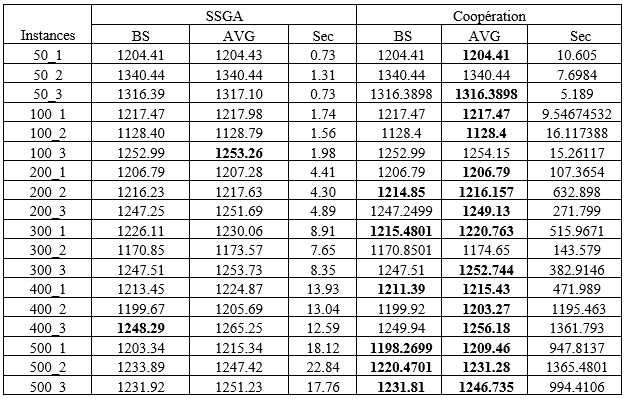
\includegraphics[width=15cm,height=8cm]{Chap5/t7.png}
	\caption{Résultats d’exécutions de SSGA et la méthode de coopération}
	\label{tab:7}
\end{table}

\end{enumerate}


\subsection{Analyse graphique}

\subsubsection{Étude comparative entre les différentes approches sur les meilleures solutions (BS) }

La Figure \ref{fig:DEAP} représente graphiquement les valeurs des différentes BS obtenues
par les méta-heuristiques  ACO\_DT, BBO, GA et la méthode coopérative, pour les 18 instances. On constate que les courbes présentent la même allure pour les instances de complexité moyenne. De plus, pour les instances de 300\_2 à 500\_3, l’approche de coopération  donne des résultats avec un coût inferieur à celui des autres approches. Chose qui prouve l’efficacité de la méthode coopérative.

\begin{figure}[H]
	\centering
	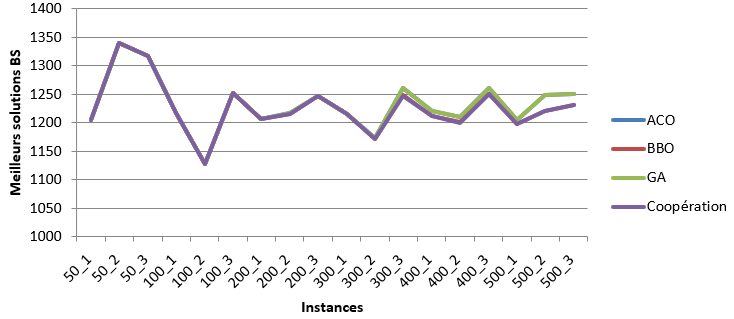
\includegraphics[width=16cm,height=7cm]{Chap5/5.png}
	\caption{Diagrammes d’exécutions des approches proposées}
	\label{fig:DEAP}
\end{figure}



\subsubsection{Comparaison de la qualité moyenne des solutions (AVG) de l’approche coopérative  et des autres approches}

La Figure \ref{fig:DQMSAP} porte sur la qualité moyenne des solutions (AVG) issues de 20 exécutions des différents algorithmes pour l’ensemble des 18 instances. On observe
que les valeurs résultantes de l’approche coopérative avoisinent celles de ACO, BBO  et GA et il est clairement aperçu que pour les grandes instances  la coopération donne de bien meilleurs résultats que les autres approches. Ceci prouve que l’approche de coopération proposée  s'adapte bien pour les grandes instances du problème. 


\begin{figure}[H]
	\centering
	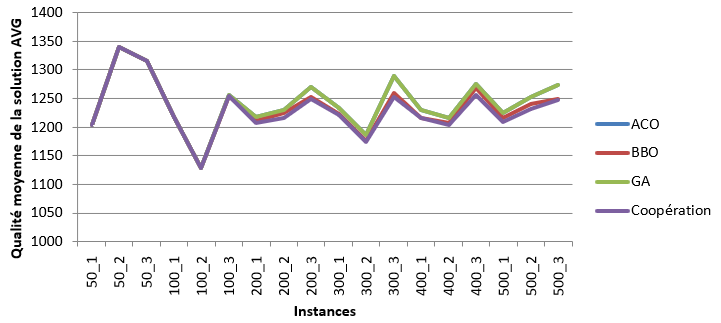
\includegraphics[width=16cm,height=7cm]{Chap5/6.png}
	\caption{Diagrammes de la Qualité moyenne de la solution AVG de des approches proposées}
	\label{fig:DQMSAP}
\end{figure}


\section{Conclusion}
A travers ce dernier chapitre, nous avons étudié les résultats expérimentaux de l’approche proposée et les avons comparées selon quelques paramètres de performances (BS,AVG), avec d’autres travaux élaborés pour la résolution du problème de l’arbre dominant. Dans l’ensemble, les approches que nous avons proposées se sont  avéré efficace en offrant de bons résultats malgré la constatation de quelques dégradations de qualité qui peut se justifier par la nature stochastique des méta-heuristiques.

